



\begin{comment}

MAIN REFS


HECKMANN\&THOMPSON, VEILLEUX ET AL 2020, ZHANG 18,

PHD THESIS GV

MAYBE SOMETHING WITH AGN FEEDBACK?


SUMMARY 


 1. INTRO: IMPORTANCE OF FEEDBACK AND LINKS WITH PREVIOUS CHAPTER
 
 1A. OBSERVATIONAL PROBES?
 
 2. DIFFERENT KIND OF OUTFLOWS: AGN-POWERED AND SF-POWERED
 
 3. DIFFERENT PHYSICAL MECHANISMS

 4. THE CC85 MODEL
 
 5. ROLE OF RADIATIVE COOLING 
 
 6. RADIATION PRESSURE POWERING OUTFLOWS
 
 7.  COSMIC RAYS POWERING OUTFLOWS
 
 8. BRIEF OVERVIEW OF THE AGN ROLE?
 
 9. SUMMARY OF WHAT WE KNOW AND WHAT WE WILL DISCOVER IN THE FUTURE
 
 
USEFUL THINGS TO MENTION
 - CC85 MODEL
 - INTRODUCING RADIATIVE COOLING \& THOMPSON'S WORK
 - 
 
\end{comment}


In 1957, the astrophysicist Eugene Parker suggested for the first time that a constant stream of particles could travel from the Sun's atmosphere to the outer regions of the Solar System due to pure hydrodynamic effects \citep{parker_wind}. This hypothesis challenged the conventional wisdom of that time, as the atmospheres of stars like the Sun were thought to be essentially in hydrostatic equilibrium. Two years later, this so-called \textit{Solar Wind} has been observed for the first time, and since then, we have become more and more aware of the ubiquity of stellar winds and of their impact on the circumstellar environment.


In the same years, "evidence for
an explosion in the center of the galaxy M82" was reported \citep{lynds_m82}: it was the first observation of gas outflowing from a galaxy. M82 has since then become the prototypical starburst galaxy, hosting a well-studied bipolar galactic wind created by SNe activity (figure \ref{fig:m82}). As authors created models for the formation of these winds on galactic scales \citep{chevalier_clegg:1985} -- using principles similar to the ones presented in the theory of stellar winds \citep{stellar_winds_holzer} -- new observations proved the presence of a greater and greater number of outflows in galaxies with different age and properties \citep{osterbrock_1960, burke_1968}. 

Today, we know that outflows are ubiquitous in starburst galaxies in the local universe, and, most importantly, in normal star-forming galaxies at medium and high redshift. As described in chapter \ref{chap:intro}, these winds are believed to play an essential role in shaping up the universe as we know it, being the main source of feedback mechanisms through which galaxies determine their own evolution. 

In this chapter, we focus entirely on the theory of galactic winds, describing their properties and their driving mechanisms. We give a brief overview of the main characteristics of outflows in section \ref{sec:intro_outflows}, exploring their nature and the information we can gain from observations. Then, we look into the theory of Supernovae-driven outflows in section \ref{sec:model_outflows}, focusing in particular on the formation mechanisms of the cold winds that are routinely witnessed in observations. 

Throughout this chapter, we will mainly follow the reviews by Veilleux et al. \citep{Veilleux:2005ia, veilleux2020cool}, Heckman \& Thompson \citep{heckman2017galactic}, Zhang \citep{zhang2018review}, and Rupke \citep{rupke2018review}. 



\begin{figure}
    \centering
    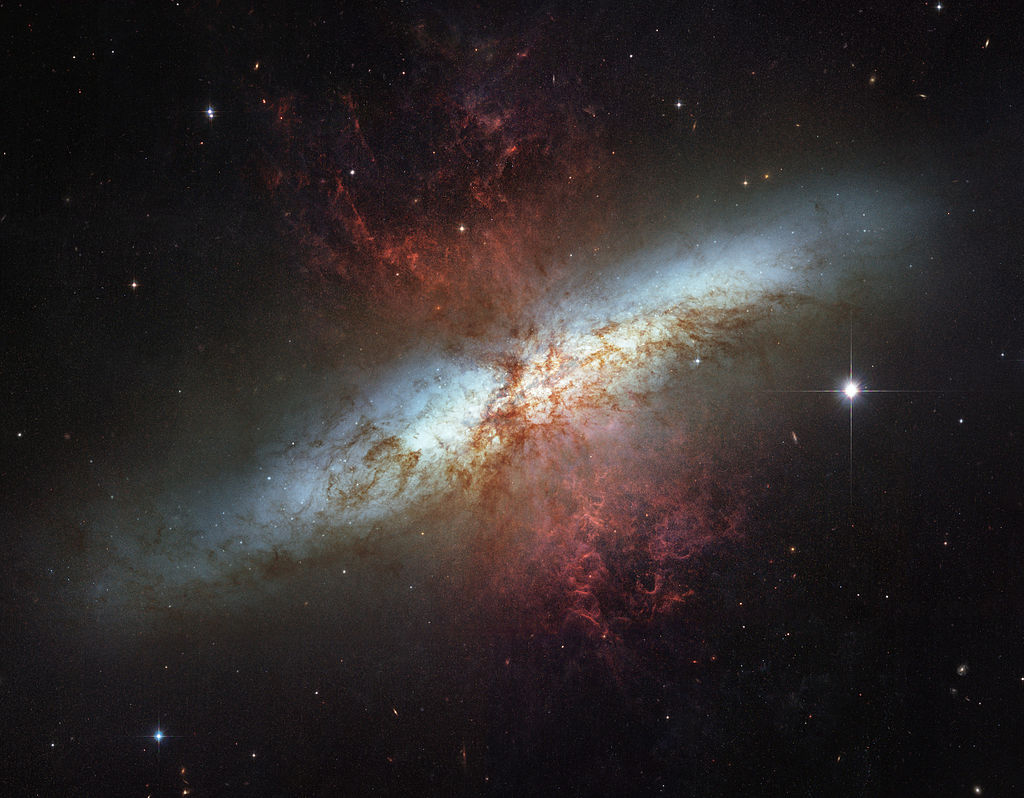
\includegraphics[width=0.58\textwidth]{plots/m82.jpg}
    \caption{Image of M82 taken by the Hubble Space Telescope (HST). The emission coming from the H$\alpha$ line (red), measured with the Subaru telescope, has been superimposed to the original HST image. Figure from the Hubble telescope
    gallery. }
    \label{fig:m82}
\end{figure}


\section{General properties} \label{sec:intro_outflows}


\subsection{Star formation and AGN driven outflows}

As already mentioned in chapter \ref{chap:intro}, outflows are thought to form both during starburst episodes (i.e., intense episodes of star formation) and during active accretion of gas on a SMBH. The former ones are driven by the energy and momentum released by stellar winds and Supernovae, while the latter ones are driven by AGN radiation or jets.

AGN feedback mechanisms are the most powerful and extreme events: for this reason, they are thought to play a relevant role in affecting the properties of even the most massive galaxies in the universe (section \ref{sec:feedback}). In the standard picture, AGN feedback is believed to operate in two different modes: a \textit{radiative} (also known as \textit{quasar}) mode and a \textit{kinetic} (\textit{radio}) mode. 

The \textit{radiative mode} is associated with very high BH accretion rates, and it is able to create powerful winds driving gas out of the galaxies \citep{silk_rees_agn}. It operates on short timescales, as the resulting strong AGN emission and powerful outflows deplete the gas reservoir in the central regions of the galaxies, quenching star formation, and, at the same time, compromising the efficiency of gas accretion on the central SMBH. Strong winds are produced in this mode thanks to the enormous amount of radiation emitted by the central AGN: the pressure associated with this radiation can accelerate a fast wind in the proximity of the SMBH. The wind - which can reach a substantial fraction of the speed of light \citep{kraemer2018physical} - impacts directly on the surrounding medium, generating a shock and thus accelerating the interstellar gas. 

\textit{Energy-driven} winds form when the shocked ISM retains its energy, expanding adiabatically on kpc scales. If the shocked gas can cool efficiently, on the other hand, a \textit{momentum-driven} wind is formed: the gas conserves its momentum but not its energy, and thus the resulting outflow is not as fast and strong as in the former scenario. We will deal with the problem of radiative cooling of the outflowing gas in section \ref{sec:outflows_cooling}. 

The \textit{kinetic mode}, instead, forms in low-luminosity AGN, where gas accretion is not as strong and the resulting radiation is not able to drive fast winds in the galaxy. This mode, however, is extremely important, as it is able to quench star formation by preventing the halo gas to accrete into the galaxy. This \textit{preventative feedback} acts by heating the CGM gas, and thus balancing the radiative cooling rate and inhibiting the ability of the gas to cool and fall into the galaxy (section \ref{sec:infall_and_cooling}). Jets, created by AGN, are thought to be responsible for this heating process thanks to their kinetic energy. This mode has large timescales, as low accretion rates on SMBHs can be sustained over longer periods of time. 

Overall, it is the combined action of radiative and kinetic mode that makes AGN feedback effective in governing the star formation rate in massive galaxies \citep{fabian12}. However, details of these processes are still lacking: despite the increasing number of AGN-powered outflows observed at low and high redshift in the last few years \citep{feruglio2010quasar, maiolino2012evidence, carniani2015ionised,Fiore_2017, cicone2018largely}, the actual mechanisms governing these outflows, as well as their impact on the host galaxies are still difficult to constraint observationally.  

Winds driven by star formation processes are in general slower and less powerful; their velocities range between a few hundred to $1000\,\kms$. For this reason, they are thought to play a major role in low-mass galaxies as well as in high redshift galaxies, where the presence of AGN becomes less common. In other respects, they are similar to the AGN radiative mode winds, but the underlying driving mechanism is different: the combined effect of stellar winds from hot stars and SNe injects into the interstellar regions hot and metal-enriched material, which can become buoyant and leave the galaxy. Note, however, that different driving mechanisms have been proposed, including radiation pressure and cosmic rays \citep[e.g.,][]{recchia_cosmic_rays, zhang_rad_pressure}.

In this work, we will focus entirely on winds driven by star formation activity: in the following sections, when not stated otherwise, we will refer to winds connected with Supernovae and hot stars. This is because our model aims to explain observations of galaxies that do not show any sign of AGN activity (chapter \ref{chap:halos}). However, in section \ref{sec:results}, we will describe how our results hint at the possibility of an obscured AGN contribution in driving outflows in the sample of galaxies considered. 




\subsection{Observational properties} \label{sec:obs_outflows}

One of the main challenges related to outflows studies is to turn observations into quantitative measurements of the basic fundamental properties of outflows. Such measurements are in fact required in order to study outflows' driving mechanisms and physical properties, and to assess how and to which extent outflows affect the central galaxy and its gas reservoir. 

The most basic quantity that is possible to infer from observations is the outflow velocity ($v$). This is because outflows are often revealed by studying absorption/emission spectral lines of galaxies. Therefore, measuring the extent of the broad-wing feature (created by the relative velocity of outflowing gas) in these lines gives a direct estimate of the wind velocity. However, contamination due to the central ISM kinematics and other similar effects can bias this measurement. In order to overcome this obstacle, different prescriptions are possible, e.g., considering only the most extreme part of the broad line component. Even though several conventions can be employed, they are broadly consistent; for this reason, the wind velocity can be considered as the most reliable quantity that can be deduced from observations. 

 
Using velocity measurements, the mass outflow rate $\dot{M}_\mathrm{out}$ can be obtained by making use of a relation based on simple dimensional analysis:
\begin{equation}
        \dot{M}_\mathrm{out} = \frac{M_\mathrm{out}v}{r_\mathrm{out}},
\end{equation}
where $M_\mathrm{out}$ is the total mass of the outflowing gas contained in a radius $r_\mathrm{out}$. In turn, the mass outflow rate can be used to compute other two relevant quantities: the kinetic energy rate ($\dot{E}_{k,\mathrm{out}} = \dot{M}_\mathrm{out}/2v^2$) and the momentum rate ($\dot{P}_\mathrm{out} = \dot{M}_\mathrm{out}v$).

Gas masses and outflow radii are quite difficult to obtain. Size measurements are possible only for spatially resolved observations. Otherwise, typical outflow sizes must be assumed, introducing a relevant source of error in the rate computation. Even when spatially-resolved observations are available, different criteria can be used to compute outflow sizes. Furthermore, the precise meaning of $r_\mathrm{out}$ inevitably depends on the particular morphology of the outflow. As for gas masses, they can be inferred by noting that the luminosity of the outflow is proportional to the volume integral of $n^2$, and hence to the product of $M_\mathrm{out}n_\mathrm{out}$. Gas densities can be measured by warm gas lines, but they depend on the ionization state and the element abundances in the gas. Therefore, measurements of outflow rates are often subject to many sources of uncertainty, and their values can be estimated only on a very coarse level.

Mass outflow rates are often parametrized also in terms of the mass loading factor $\eta = \dot{M}_\mathrm{out}/\mathrm{SFR}$. Assuming mass conservation in the outflow, this quantity can also be described as the ratio between the rate of ISM gas mass that is loaded in the outflow and the star formation rate. This quantity plays a relevant role in the context of feedback mechanisms and star formation quenching, as high values of $\eta$ imply that fraction of ISM gas that is expelled from the galaxy is higher than the one that contributes to forming stars. This can ultimately lead the galaxy to run out of gas, quenching any subsequent SF activity (section \ref{sec:feedback}). The mass loading factor will play a key role in subsequent chapters.

\subsection{The multiphase nature of galactic winds} \label{sec:multiphase}



The picture emerging from outflows' observations is complex and difficult to interpret. In particular, it has been thoroughly proved by multi-wavelength surveys that outflowing gas hosts a wide variety of thermodynamical conditions: hot and highly ionized gas is often mixed with cold, neutral, or even molecular gas. This fact represents one of the greatest theoretical and observational challenges linked with the physics of outflows, as it poses a range of questions whose answers are still far from clear:
\begin{itemize}
    \item Which is the relative contribution of the different phases to the energy, mass, and metals budget of the outflow?
    \item Provided that the driving mechanism for SN-driven winds is effective only for hot gas, how is the colder gas formed in the outflow? 
    \item Do different phases have different physical properties and live on different scales?
    \item How do different phases affect the host galaxy via feedback effects? 
\end{itemize} 
Furthermore, observations of outflows are much more difficult in light of their complex nature. Since winds are studied using either emission or absorption spectral lines, individual observations typically give information only on a specific phase, and not on the properties of outflows as a whole. This often hinders a precise assessment of the outflows' role in driving galaxy evolution (see section \ref{sec:feedback}). 


Conventionally, five different phases can be identified, based on the temperature of the gas (or, equivalently, on its ionization state, as the ionization of gas depends primarily on its temperature): a very hot phase ($T\sim 10^8\,\mathrm{K}$), a hot and highly ionized phase ($T\sim 10^{6-7}\,\mathrm{K}$), a warm and ionized phase ($T\sim 10^{4-5}\,\mathrm{K}$), a cool and neutral atomic phase ($T\sim 10^3\,\mathrm{K}$), and a cold and molecular/dusty phase ($T\sim 10-100\,\mathrm{K}$). Each phase can be traced by a different set of species, given that the presence of those species depends on the temperature of the gas. For example, very hot gas will emit in the X-ray, and thus X-ray emission and absorption features can be used to constraint the properties of the gas hot phase \citep{Strickland:2000jg, strickland2009supernova}. In a similar way, ionized species such as \OIII are tracers for the warm phase at $10^4\,\mathrm{K}$, while species such as \CIIion, \HI, \HH, CO trace the atomic neutral and molecular phases. 

Using these tracers, observations tend to agree on the fact that hot outflows are fast ($v\approx 1000\,\kms$) and dominate the kinetic energy budget of the outflowing material. Cold/warm neutral outflows, on the other hand, are found to dominate the total mass outflow rate, and they are often slower, with velocities in the range $v\approx 100-500\,\kms$ \citep[e.g.,][]{rupke2013multiphase}.


\section{Models for star formation driven outflows} \label{sec:model_outflows}

In this section, we review the theory of galactic outflows driven by star formation, by looking at the most important models that have been proposed to explain the formation and evolution of galactic-scale winds. A satisfactory theoretical explanation for the origin of these outflows cannot neglect the observational properties that outflows present at low and high redshifts. 

As described in the last section, the most striking feature of outflows is the presence of many different phases, ranging from the very hot gas to the cold molecular one. The key question is then how these phases are formed within the outflow, and how they evolve over different spatial and time scales. We start by considering the classical model for hot outflowing gas, first proposed by Chevalier \& Clegg in 1985 \citep{chevalier_clegg:1985} (hereafter, CC85). Then, we focus on the warm and cool phases by analyzing gas radiative cooling and the acceleration of the cool gas by the outflowing wind.  



\subsection{CC85 model} \label{sec:cc85_model}

The CC85 model describes a hot and steady wind that drives gas out from the center of the galaxy. The wind is created by the energy and mass released by overlapping Supernovae events. Despite the fact that describing the physical processes leading to the formation of winds from SNe is extremely complex, simple analytical estimates can be applied on galactic scales, where the properties of single events are averaged. In particular, a constant rate of energy and mass injection in the gas is assumed inside the galaxy, modeled as a sphere of radius $R$. 

With these assumptions, the configuration is time-steady and spherically symmetric. In the region inside the sphere of radius $R$, mass and energy are not conserved: we call the source terms $\dot{M}$ and $\dot{E}$ respectively. Outside the spherical region, instead, the gas is assumed to expand adiabatically, conserving both mass and energy. This is a key assumption, as it means that any radiative loss is neglected in the outflow: we will later revise this hypothesis when dealing with cool gas formation. Thermal conductivity and viscosity are neglected as well. Moreover, gravitational effects are considered to be small, since, as we will prove in a moment, the velocity at the edge of the galaxy is much greater than the escape velocity of the gas. 

With these conditions, we can write the two equations for hydrodynamics (mass conservation and Euler equation), closing the system with the energy conservation equation:
\begin{subequations}
\begin{align}
    &\pder{\rho}{t} +\mathbf{\nabla} \cdot (\rho \mathbf{v})=q\\
    &\pder{\mathbf{v}}{t} + (\mathbf{v}\cdot \mathbf{\nabla})\mathbf{v} = - \frac{1}{\rho}\mathbf{\nabla} \cdot P - \mathbf{v}q\\
    &\pder{}{t}\bigg(u+\rho\frac{v^2}{2}\bigg)+\mathbf{\nabla}\cdot\bigg(\mathbf{v}\bigg(h+\rho \frac{v^2}{2}\bigg)\bigg)=Q
\end{align}
\end{subequations}
In these expressions, $\rho, v, p$ are the gas density, velocity, and pressure respectively; $u$ is the internal energy density per unit volume, while $h$ is the enthalpy per unit volume ($h=u+P$). Using the definition of the internal energy ($u=(\gamma -1)^{-1}nkT$), as well as gas equation of state (eq. \ref{eq:state_equation}), we can rewrite the enthalpy as: 
\begin{align}
   h = \frac{\gamma}{\gamma -1} \,P,
\end{align}
where $\gamma = 5/3$ is the adiabatic index.

The mass input rate $q$ and energy input rate $Q$ per unit volume - assumed to be constant in space and time - take the form:
\begin{equation}
\begin{cases} q=\frac{3\dot{M}}{4\pi R^3}\,, \,\,\,r\le R\\ q=0\,, \,\,\,r> R \end{cases}
\qquad \begin{cases} Q=\frac{3\dot{E}}{4\pi R^3}\,, \,\,\,r\le R\\ Q=0\,, \,\,\,r> R \end{cases}
\end{equation}

With these definitions, we can search for a steady-state solutions by dropping the partial time derivative terms. Using spherical coordinates, we get:
\begin{subequations} \label{eq:eul_cc85}
\begin{align}
&\frac{1}{r^2}\der{}{r}(r^2v\rho)=q  \label{eq:eul1_cc85}\\
&\rho v\der{v}{r}= -\der{p}{r} -vq \label{eq:eul2_cc85}\\
&\frac{1}{r^2}\der{}{r}\bigg[r^2\rho v\bigg( \frac{v^2}{2}+\frac{\gamma}{\gamma -1}\frac{p}{\rho}\bigg)\bigg]=Q, \label{eq:eul3_cc85}
\end{align}
\end{subequations}

Imposing appropriate boundary conditions for the system $v(0)=0$, $\rho(r\rightarrow+\infty)=T(r\rightarrow+\infty)=0$, we can solve the equations in the two regions. By requesting a smooth transition between the two solutions, we find that this model describes an outflow transitioning from a sub-sonic regime in the inner region to a super-sonic adiabatic expansion in the outer one. The general solution can thus be conveniently expressed in terms of the Mach number $\mathcal{M} = v /c_s$, which is defined by considering the sound speed of the gas:
 \begin{align}
   c_s^2 =\gamma\,\frac{P}{\rho} = \gamma\, \frac{k_B}{\mu m_p} T \label{eq:sound_speed}
 \end{align}
 The solutions in the two regions, then, reads: 
\begin{align}
&\bigg(\frac{3 \gamma + 1/\mathcal{M}^2}{1+3 \gamma}\bigg)^{-(3\gamma+1)/(5 \gamma+1)}\bigg(\frac{\gamma-1+2/\mathcal{M}^2}{1+\gamma}\bigg)^{(\gamma+1)/(2(5\gamma+1))} = \frac{r}{R} \label{eq:solinn}\\
&\mathcal{M}^{2/(\gamma-1)}\bigg(\frac{\gamma-1+2/\mathcal{M}^2}{1+\gamma}\bigg)^{(\gamma+1)/(2(\gamma-1))} = \bigg(\frac{r}{R}\bigg)^2 \label{eq:solout}\,,
\end{align}
where eq. \ref{eq:solinn} (eq. \ref{eq:solout}) applies to $r<R$ ($r>R$). To grasp the properties of these solutions, it is useful to introduce dimensionless variables ($r_*$, $v_*$, $\rho_*$, and $P_*$) using the input quantities $R$, $\dot{M}$, $\dot{E}$, as a unit radius, mass rate, and energy rate respectively:
\begin{subequations} \label{eq:dimensionless_cc85}
\begin{align}
    &r = r_* \,R\\
    &v = v_*\,\dot{E}^{1/2}\,\dot{M}^{-1/2}\\
    &\rho = \rho_*\,\dot{E}^{-1/2}\,\dot{M}^{3/2}\,R^{-2}\\
    &P = P_*\,\dot{E}^{1/2}\,\dot{M}^{1/2}\,R^{-2}
\end{align}
\end{subequations}
Figure \ref{fig:cc85} shows the profiles for the dimensionless parameters $v_*$, $\rho_*$, and $P_*$, as a function of the dimensionless radius $r_*$. As already noted, the solution represents an outflow undergoing a sonic transition (i.e., $\mathcal{M} = 1$) at $r_* = 1$: for smaller radii, the velocity increases monotonically, while density and pressure slowly decrease; near the sonic point, profiles steepen as they present a divergence in the first derivative at $r_*=1$. Then, the flow transitions to a super-sonic adiabatic expansion, with the velocity reaching an asymptotic value, and the pressure and density decreasing with a power-law scaling. Numerical estimates of these scalings can be easily determined considering eqs. \ref{eq:eul_cc85}: in the outer region $Q=q=0$, hence mass conservation yields $\rho v r^2 = \mathrm{const.}$, while energy conservation can be recast in the form of a Bernoulli integral conservation: 
\begin{align}
 B = \frac{v^2}{2} + \frac{\gamma}{\gamma -1}\,\frac{P}{\rho} = \mathrm{const.} = \frac{\dot{E}}{\dot{M}}, \label{eq:bernoulli}
\end{align}
where the last equality can be inferred simply noting that the Bernoulli integral represents the total energy per unit mass of the fluid. At infinity, the second term in eq. \ref{eq:bernoulli} vanishes: we then find $v_\infty = \sqrt{2}\,\dot{E}^{1/2}\,\dot{M}^{-1/2}$ (i.e., $v_{*,\infty} = \sqrt{2}$). Knowing that the velocity in asymptotically constant, we easily infer that density scales as $\rho\sim r^{-2}$ to conserve the mass; hence, pressure and temperature scales as $r^{-2\gamma}$ and $r^{-2(\gamma-1)}$, as the adiabatic equation holds ($P\rho^{-\gamma}=\mathrm{const.}$). 

Numerical values at the sonic point ($v(R)$, $\rho(R)$, $P(R)$) can be determined simply considering eq. \ref{eq:bernoulli}, setting $v=c_s$ ($\mathcal{M}=1$), and integrating eq. \ref{eq:eul1_cc85} in the inner zone:
\begin{subequations}
\begin{align}
    &v_*(R) = \left(\frac{1}{2}+\frac{1}{\gamma-1}\right)^{-1/2}\label{eq:bound_cc85_1}\\
    &\rho_*(R) = \frac{1}{4\pi v_*}\\
    &P_*(R) = \frac{v_*}{4\pi \gamma}\label{eq:bound_cc85_3}
\end{align}
\end{subequations}

The physical relevance of the CC85 model can be appreciated by setting some reasonable input values for the mass and energy inputs. As already described in section \ref{sec:feedback}, the energy input from SNe can be parametrized by introducing the energy released by a single SN ($E_{0,\mathrm{SN}}$) and the frequency of SNe per unit mass $\nu_\mathrm{SN}$. We choose $E_{0,\mathrm{SN}} = 10^{51}\,\mathrm{erg}$ \citep{ostriker_supernovae} and $\nu_\mathrm{SN} = 10^{-2}\,\msun^{-1}$ (this holds true for a Salpeter IMF \citep{leitherer1999}, see also sec. \ref{sec:star_formation}). With these parameters, both the energy and the mass input rates can be expressed as a linear function of the star formation rate. We introduce two efficiency factors, the thermalization efficiency $\alpha$ and the mass loading factor $\eta$ (seec. \ref{sec:obs_outflows}), to parametrize the coupling between SNe ejecta and the outflowing gas:
\begin{subequations}
\begin{align}
    &\dot{E}=\alpha  E_{0,\mathrm{SN}} \nu_\mathrm{SN} \,\mathrm{SFR}\\
    & \dot{M}=\eta \, \mathrm{SFR}
\end{align}
\end{subequations}

With these choices for the input parameters, the terminal velocity of the outflow is independent of the SFR: $v_\infty \approx 10^3\,\mathrm{km}\,\mathrm{s}^{-1} \,( \alpha / \eta )^{1/2}$. For values of $\alpha$ and $\eta$ close to unity, this velocity is much greater than the circular velocity of galaxies, hence gravity does not play a relevant role in the model. When examining radiative cooling outflows, this hypothesis will not hold true, as the outflows slow down because of thermal losses and they are affected by the halo gravitational potential (section \ref{sec:cooling_gravity}). 

Other useful quantities are the temperature and density at the critical point $r=R$:
\begin{subequations}
\begin{align}
    & T(R) \approx 2\times10^7\,\left(\frac{\alpha}{\eta}\right)\\
    & n(R) \approx 1\times10^{-2}\,\mathrm{cm}^{-3}\,\left(\frac{\mathrm{SFR}}{1\,\msun\,\mathrm{yr}^{-1}}\right) \left(\frac{R}{1\,\mathrm{kpc}}\right)^{-2}\,\left(\frac{\eta^{3/2}}{\alpha^{1/2}}\right)
\end{align}
\end{subequations}
These quantities will play an important role in subsequent discussion (chapter \ref{chap:model}). 

Overall, the CC85 model describes an outflow with high temperature, relatively low density, and high terminal velocities. These quantities are compatible with X-rays observations of the hot phases of outflows in local starburst galaxies: estimates of the two efficiency parameters from these observations hold $\alpha=0.3-1$, $\eta=0.2-0.6$  \citep[e.g.,][]{strickland2009supernova, zhang2014hot}. 

This model has thus become the standard way to approach the problem of adiabatic hot flows. Several works have confirmed the main results of the model in numerical hydrodynamical simulations, both in idealized setups \citep{Strickland:2000jg} and in realistic 3d cases \citep{cooper2009starburst, schneider2018production}. Variations on the model have also been proposed: for instance, Bustard et al. \citep{bustard2016versatile} have considered a more realistic non-uniform profile for the input region, also including the contribution of the galaxy gravitational potential. They have shown that in this less idealized scenario the non-physical divergence in the first derivative of thermodynamical variables disappears, and the sonic point does not coincide with the edge of the galaxy for a general mass input profile. However, quantitative conclusions for the CC85 model hold true even in this case: the only approximation that ceases to be valid for some values of the input parameters is that the outflow evolves adiabatically. In the next section, we will focus on this approximation, describing how a hot flow is able to cool down thanks to radiative losses, and how this impacts the subsequent evolution of the wind.  




\begin{figure}
    \centering
    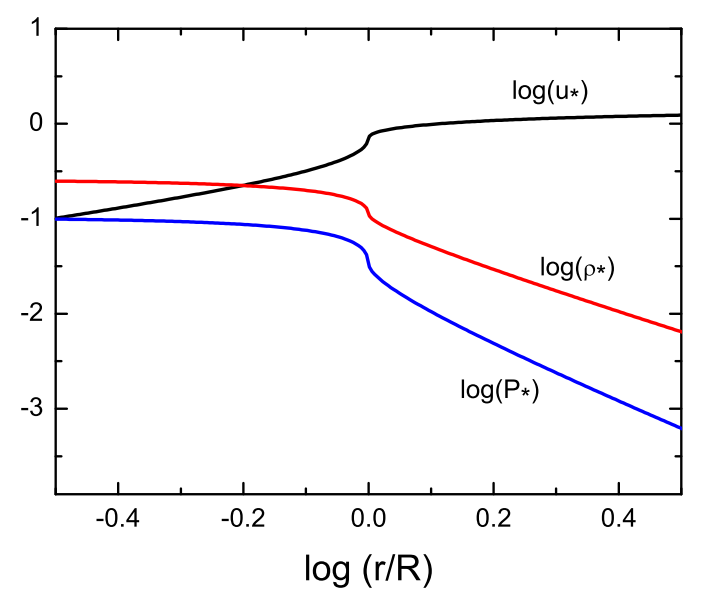
\includegraphics[width=0.5\textwidth]{plots/cc85.PNG}
    \caption{Radial solutions for the CC85 model \citep{chevalier_clegg:1985}. The black, red, and blue lines show the profiles for the dimensionless parameters $u_*$, $\rho_*$, and $P_*$ (eqs. \ref{eq:dimensionless_cc85}) respectively, as a function of the dimensionless radius $r_*=r/R$. Figure taken from \citet{zhang2018review}.
    }
    \label{fig:cc85} 
\end{figure}




\subsection{Cold flows and related problems}\label{sec:outflows_cooling}


While the physics underlying the formation and evolution of hot flows is well established, the presence of cold gas outflowing at high speed (hundreds of $\kms$) from galaxies has represented a formidable theoretical problem in the last two decades. The fundamental question that needs to be answered is how to accelerate cool atomic and warm ionized gas to these velocities, as the cold gas is not buoyant and thus is not able to form a wind on its own. Two mechanisms have gained momentum in the literature: in the first one, the ram pressure of hot outflowing gas accelerates the cold ISM, creating a cool phase in the outflow; in the second one, hot gas cools by emitting radiation and thus forming a warm (and possibly cool) uniform phase. We will review both these explanations in the next paragraphs, as they will be relevant in the development of our model in the following chapters. 


\subsubsection{Acceleration of warm/cool clouds in hot winds}

According to the first mechanism, cold gas in outflows comes from ISM material that is accelerated and entrained in the hot wind. The factor that is responsible for accelerating the gas is generally identified in the ram pressure of the hot flow (however, other driving mechanisms are possible, e.g., radiation pressure on dust). In fact, since the hot outflow is highly supersonic in the external region (eq. \ref{eq:solout}), its ram pressure is much greater than its thermal pressure, and thus it can transfer momentum to the cold material in the ISM driving it to velocities as high as thousands of $\kms$. 

A good estimate for this momentum exchange rate can be obtained by considering a simple model of a uniform spherical cold cloud at rest in a flow of hot gas with velocity $v_\mathrm{hot}$ and density $\rho_\mathrm{hot}$. Defining the radius of the cloud $R_c$ and its density $\rho_c$, one can equate the force acting on the cloud because of the flow's ram pressure $\rho_\mathrm{hot}\,v_\mathrm{hot}^2 \,\pi\,R_c^2$ to the rate of change of the cloud momentum. The acceleration timescale $t_\mathrm{acc}$ in which the cloud's velocity reaches $v_\mathrm{hot}$ is then:
\begin{align}
       \tau_\mathrm{acc} = \frac{4R_c}{3v_\mathrm{hot}}\,\frac{\rho_c}{\rho_\mathrm{hot}}
\end{align}
We can get a rough estimate for this timescale considering the typical radius for a cloud $R_c \sim 100\,\mathrm{pc}$, and setting the temperature of the cloud to $T_c \sim 10^4\,\mathrm{K}$ (i.e., the equilibrium value at which photoheating balances radiative cooling; see section \ref{sec:cooling_function}). At this temperature, the Jeans scale of the cloud is much greater than $R_c$ for a wide range of densities. Hence, the cloud must be pressure-confined by the hot medium: for this reason, the density ratio $\rho_c/\rho_\mathrm{hot}$ is equal to the inverse of the temperature ratio $T_\mathrm{hot}/T_c$. According to the CC85 model, the hot medium has a temperature of $T_\mathrm{hot}\sim 10^7\,\mathrm{K}$ near the boundary region $r=R$; we thus get $\rho_c / \rho_\mathrm{hot} \sim 10^3$. Further setting $v_\mathrm{hot} \approx 10^3 \,\kms$ in adherence to CC85, we find that the acceleration time scales as $\tau_\mathrm{acc}\approx 100\,\mathrm{Myr}\, (R_c/100\,\mathrm{pc})$. In principle, since this timescale is smaller than the Hubble time, this acceleration mechanism could be responsible for creating the cold phase in galactic winds.

However, this estimate does not take account of the disruptive effect the hot flow has on the cloud. In fact, as the supersonic wind encounters the cloud at rest, it drives a shock into the overdense gas. The velocity with which this shock travels inside the cloud, $v_s$, can be determined by using the following argument (for more details, see \citep{klein_1994, scannapieco2015launching}): if the shock is highly supersonic, then the pressures on the two sides of the shock are approximately equal. The post-shock pressure is $\rho_\mathrm{hot}\,v_\mathrm{hot}^2$, while the pressure behind the shock (inside the cloud) is $\rho_c \,v_s^2$. Equating these two quantities, we get an expression for the velocity of the shock:
\begin{align}
    v_s = v_\mathrm{hot}\,\left(\frac{\rho_\mathrm{hot}}{\rho_c}\right)^{1/2}
\end{align}
Thus, we can introduce another important timescale, the \textit{cloud-crushing time} $t_{cc}$, by considering the time it takes the shock to travel through the cloud, heating and disrupting it in the process. Using the expression for $v_s$, we find:
\begin{align}
    t_{cc} \sim \frac{R_c}{v_s} \sim \frac{R_c}{v_\mathrm{hot}}\,\left(\frac{\rho_c}{\rho_\mathrm{hot}}\right)^{1/2}
\end{align}
As the cloud is heated and shredded by the shock, we expect that its complete destruction happens in a few cloud-crushing times: this was proven using hydrodynamical simulations as early as 1994 by Klein et al. \citep{klein_1994}. In figure \ref{fig:cloud_crushing}, we show a more recent simulation by Schneider \& Robertson \citep{schneider2017hydrodynamical} of a $10\,\mathrm{pc}$ cloud being disrupted by the hot flowing gas. 

If we compare the cloud-crushing time with the acceleration time, we note that, as long as $\rho_c\gg\rho_\mathrm{hot}$, $\tau_{cc}\ll\tau_\mathrm{acc}$. This poses a serious issue to the theory of accelerating clouds, as it predicts that clouds are always disrupted and incorporated into the hot wind before they can be accelerated to the velocities usually measured by observations. In order to solve this problem, several works have focused on taking into account different physical processes that are usually neglected in the basic picture: in particular, the presence of radiative cooling, thermal conduction, and magnetic fields have been proven to prolong the clouds lifetime. 

Radiative cooling allows the cold gas to survive longer as it can quickly radiate away the thermal energy gained by the interaction with the shock wave. If cooling is efficient, then the cloud can survive the shock, but it is nevertheless destroyed in a time proportional to $\tau_{cc}$ by hydrodynamical instabilities. Simulations show that this destruction timescale is dominated by shear instabilities and scales as $t_{cc}\,\sqrt{1+\mathcal{M}_\mathrm{hot}}$ \citep{scannapieco2015launching}. 

Thermal conduction driven by free streaming electrons in the hot flow also plays a relevant role: as shown by a number of works \citep[e.g.,][]{bruggen2016launching}, the outer layers of the cloud evaporates because of conduction; the core regions, instead, are stretched into dense and cold filaments, in a process that has the overall effect of stabilizing the cloud against hydrodynamical instabilities. These cold filaments, however, have a smaller cross-section with the hot flow, and therefore they are accelerated less efficiently by the wind. Finally, magnetic fields have been shown to significantly increase both the lifetime of the cloud and the drag force accelerating it \citep{mccourt2015magnetized}.

Although the combined effect of these processes could in principle extend the lifespan of cold gas and account for the cold phase observed in multiphase galactic winds, it remains unclear whether this picture is realistic enough, as simulations are efficient only in describing very idealized setups. Overall, the problem of how to accelerate cold ISM material driving it to a substantial fraction of the hot phase's velocity remains yet to be solved. For this reason, a different explanation for the cold phase of galactic winds has been proposed: in this alternative scenario, the cold phase precipitates directly from the hot flow because of radiative cooling. We examine the physics involved in this mechanism in the next paragraph.




\begin{figure}
    \centering
    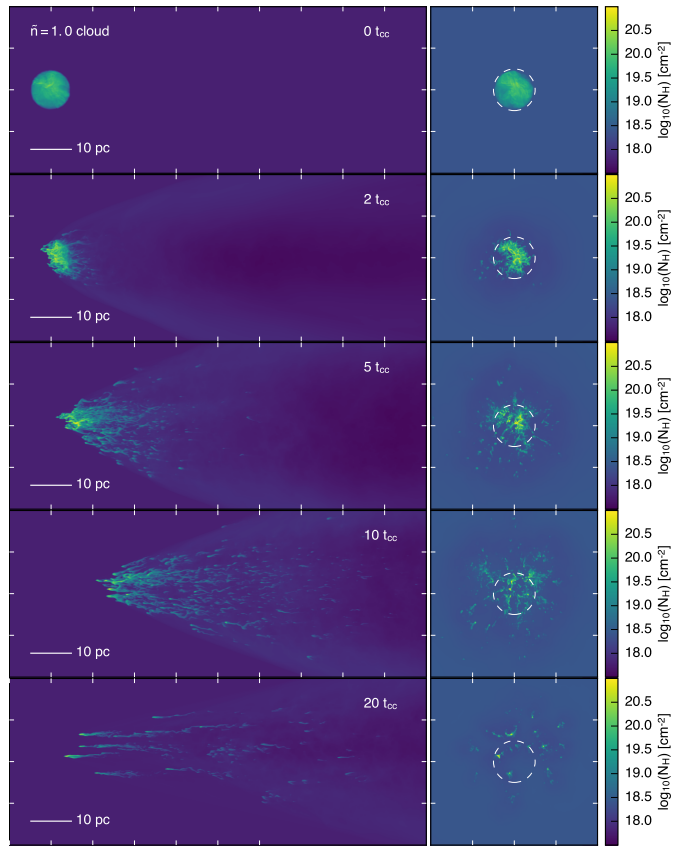
\includegraphics[width=1.0\textwidth]{plots/cloud_crushing.PNG}
    \caption{Time series evolution of a turbulent cloud entrained in a hot flow. Plots on the left show the surface density projected along the y-axis, with the wind entering the box from the left, while the right column shows the surface density projected in the direction of the wind velocity. Snapshots are shown at $t = 0, 2, 5, 10,$ and $20\,t_{cc}$. Cooling is included in the simulation: this allows the cloud to survive for around $10\,t_{cc}$ before being disrupted by the hydrodynamical instabilities. Taken from Schneider \& Robertson \citep{schneider2017hydrodynamical}.
    }
    \label{fig:cloud_crushing}
\end{figure}


\subsubsection{Radiatively cooling outflows} \label{sec:thompson_model}


In 1995, Wang \citep{Wang:1995} was the first one to point out that gas in the CC85 model can radiate a non-negligible amount of energy, and thus the wind can significantly depart from a simple adiabatic evolution in the region outside of the galaxy. This possibility has been widely studied by a number of different works, both in the context of galaxies \citep{McCourt:2015, sarkar:2015, Thompson16, Scannapieco:2017, Schneider:2018, Gronke&Oh:2020, fielding2021} and super-star clusters (SSC) \citep{Silich:2004, tenorio2003supergalactic, tenorio2007hydrodynamics, gray2019catastrophic, danehkar_2021}.


As pointed out by Thompson et al. \citep{Thompson16}, it can be proven that CC85-like highly mass-loaded winds inevitably cool on large scales. The reason for this can be inferred by comparing the cooling timescale $\tau_\Lambda$ (eq. \ref{eq:tcool}) with the \textit{advection time} $\tau_\mathrm{adv} = r / v(r)$ (i.e., the time it takes a fluid element to travel a unit distance). The discussion here echoes the study of the accretion mechanisms of the halo gas on the galaxy (section \ref{sec:accretion}): if the cooling timescale is longer than the advection time, then the evolution of the wind can be considered adiabatic, because the fluid element is brought to large distances from the galaxy before it is able to radiate away its energy. As the cooling timescale becomes shorter than the advection time, the evolution can depart significantly from the adiabatic one: cooling becomes suddenly very efficient, and the gas temperature drops abruptly in a process known as \textit{catastrophic cooling}. 
%We will describe this process in greater detail in chapter \ref{chap:model}, as it constitutes the core of the model we develop in this work. 

In order to study the conditions for which radiative cooling starts to become efficient, we have to look at the temperature dependence of the cooling function of the gas $\Lambda^\mathrm{(cool)}(T)$: this quantity is defined as $\Lambda^\mathrm{(cool)}(T) = \dot{\varepsilon}/n^2$, where $\dot{\varepsilon}$ is the rate of radiative losses per unit volume.  Note that we are focusing only on the temperature dependence of $\Lambda^\mathrm{(cool)}$ because the cooling function is independent of the gas density in the low density limit (section \ref{sec:gas_cooling_heating}); furthermore, we are neglecting further dependences on the metallicity, on the radiation fields acting on the gas, etc., because in this context we are only interested in very crude estimates. If the temperature is greater than about $10^7\,\mathrm{K}$, the processes that dominate emission are free-free collisions (\textit{bremsstrahlung}): these processes have a temperature dependence that scales as $\dot{\varepsilon}_{ff}\sim T^{1/2}$. Therefore, the cooling timescale reads (see also eq. \ref{eq:tcool}):
\begin{align}
    \tau_\Lambda = \frac{1}{\gamma - 1}\frac{\mu m_p k_B T}{\rho(r)\Lambda^\mathrm{(cool)}(T)} \sim \frac{T^{1/2}}{\rho}
\end{align}
We can express the radial dependence of these variables by supposing that the flow starts adiabatic, and using the scalings of a pure adiabatic expansion as dictated by the CC85 model in the limit of great galactocentric distances (i.e., $r\gg R$): we take the velocity as a constant, while the density decreases as $r^{-2}$ and the temperature as $r^{-4/3}$ (again, we consider $\gamma = 5/3$). Hence, the cooling timescale depends on the radius as $\tau_\Lambda\sim r^{4/3}$. Since $\tau_\mathrm{adv} = r/v \sim r$, the ratio between the cooling and the advection times slowly grows with radius: $\tau_\Lambda/\tau_\mathrm{adv}\sim r^{1/3}$. Therefore, if the flow starts adiabatic and the temperature does not drop under $10^7\,\mathrm{K}$, radiative losses can always be neglected and the entire evolution follows the CC85 model.

Things change when we consider lower temperatures: in the range $10^5\,\mathrm{K}\,\lesssim T\lesssim\, 10^7\,\mathrm{K}$, atomic line emission starts to dominate the cooling function. The temperature dependence in this range can be roughly approximated by a power-law of the form \citep{mac_low_cooling} (valid for solar metallicity):
\begin{align}
    \Lambda^\mathrm{(cool)}(T) = 3\times10^{-23}\,\left(\frac{T}{10^7}\right)^{-0.7}\,\mathrm{erg}\,\mathrm{cm}^3\,\mathrm{s}^{-1}
\end{align}
Thus, in this regime, the cooling time scales as $\tau_\Lambda\sim r^{-4/15}$ and the ratio $\tau_\Lambda / \tau_\mathrm{adv}$ is a steep decreasing function of radius ($\tau_\Lambda / \tau_\mathrm{adv} \sim r^{-19/15}$). For this reason, even if the flow starts adiabatic, there exists a radius $r_\mathrm{cool}$ for which the cooling time gets lower than the advection time. Outward of $r_\mathrm{cool}$, radiative losses are important and the wind rapidly cools down to lower temperature, significantly departing from the adiabatic evolution as the flow slows down and the density tends to increase. 

We can study the importance of these cooling effects by computing the radius $r_\mathrm{cool}$ and comparing it with the size of the galaxy $R$. Again, we work in the asymptotic regime for which $r\gg R$: taking this limit in the solution for the CC85 model (eq. \ref{eq:solout}), we infer the values of $v_\infty$, $T_\infty(r)$, and $\rho_\infty(r)$. Given these quantities, the resulting timescales are: 
\begin{subequations}
\begin{align}
    & \tau_\Lambda \approx 3\times10^6\,\mathrm{yr}\,\left(\frac{\alpha^{2.20}}{\eta^{3.20}}\right)\,\left(\frac{r}{10\,\mathrm{kpc}}\right)^{-0.27}\,\left(\frac{R}{0.3\,\mathrm{kpc}}\right)^{2.27}\,\left(\frac{\mathrm{SFR}}{10\,\msun\mathrm{yr}^{-1}}\right)^{-1}\,\mu \\
    & \tau_\mathrm{adv} \approx 10^7\,\mathrm{yr}\,\left(\frac{\eta}{\alpha}\right)^{0.5}\,\left(\frac{r}{10\,\mathrm{kpc}}\right)
\end{align}
\end{subequations}
From these scalings, we can infer that the cooling radius has a very strong dependence both on $\alpha$ and on $\eta$. In particular, it critically depends on the mass loading factor $\eta$, whose importance will become clear in section \ref{sec:outflow_model}.
\begin{align}
    r_\mathrm{cool} \approx 4\,\mathrm{kpc}\,\frac{\alpha^{2.13}}{\eta^{2.92}}\,\mu^{0.79}\,\left(\frac{R}{0.3\,\mathrm{kpc}}\right)^{1.79}\,\left(\frac{\mathrm{SFR}}{10\,\msun\mathrm{yr}^{-1}}\right)^{-0.79} \label{eq:rcool}
\end{align}
Note that this discussion is valid for a gas temperature in the range $10^5-10^7\,\mathrm{K}$. According to the CC85 model (for $\alpha$ and $\eta$ close to unity), the gas temperature starts higher than $10^7\,\mathrm{K}$ and evolves adiabatically scaling as $r^{-4/3}$. For this reason, our estimate of $r_\mathrm{cool}$ is meant to be only a rough approximation, as it neglects the presence of an internal region where cooling via bremsstrahlung is inefficient. More importantly, our argument does not take into account the possibility that the gas stays adiabatic until the temperature gets lower than $10^5\,\mathrm{K}$. If this happens, then radiative cooling becomes inefficient again (because the cooling function drops at $T\sim10^4-10^5\,\mathrm{K}$, sec. \ref{sec:cooling_function}) and the evolution just proceeds according to the CC85 model: in this case, our estimate of $r_\mathrm{cool}$ does not contain any physical meaning. We can restate this reasoning by providing a minimum value of $\eta$ for which $r_\mathrm{cool}$ falls into the region of the CC85 profile where the temperature is greater than the $10^5\,\mathrm{K}$ threshold. A simple calculation gives:
\begin{align}
    \eta_\mathrm{min} \approx 0.64\,\alpha^{0.636}\,\left(\frac{R}{0.3\,\mathrm{kpc}}\right)^{0.364}\,\left(\frac{\mathrm{SFR}}{10\,\msun\mathrm{yr}^{-1}}\right)^{-0.364}
\end{align}
For $\eta \lesssim \eta_\mathrm{min}$, the wind is adiabatic until arbitrarily large radii, since $\tau_\Lambda/\tau_\mathrm{adv}$ stays always above one. As $\eta$ increases, cooling starts to become efficient, and $r_\mathrm{cool}$ becomes smaller and smaller until it becomes comparable to $R$. For these high values of the mass loading factor, our approximation $r\gg R$ fails, and thus we have to compute the cooling radius using the full CC85 solutions for the $\rho(r)$ and $T(r)$ profiles. We can consider the limit for which $r_\mathrm{cool} = R$; in this case, the corresponding value of the mass loading factor $\eta_\mathrm{crit}$ is:
\begin{align}
    \eta_\mathrm{crit} \approx 1.35\,\alpha^{0.730}\,\left(\frac{R}{0.3\,\mathrm{kpc}}\right)^{0.270}\,\left(\frac{\mathrm{SFR}}{10\,\msun\mathrm{yr}^{-1}}\right)^{-0.270} \label{eq:eta_crit}
\end{align}
As $\eta$ approaches $\eta_\mathrm{crit}$, the cooling radius gets closer and closer to the boundary region $r=R$. This suggests considering the effects of radiative cooling also for $r<R$ (i.e., inside the galaxy), where mass and energy are deposited according to the CC85 model. A number of different works have dealt with this problem, showing that for $\eta \lesssim \eta_\mathrm{crit}$ radiative cooling is efficient in the central region of the galaxy, and that rapidly cooling gas does not take part in the outflow, effectively lowering the mass loading factor \citep[for details, see][]{tenorio2007hydrodynamics, lochhaas2021characteristic}. However, these conclusions are strongly influenced by the mass and energy injection profiles, which are extremely simplistic in the original CC85 approach. Moreover, the mass loading factor is affected also by the complex interaction between the ISM and the hot supernovae ejecta; the assumption of stationarity for the flow may cause some issues when dealing with cooling in the internal region of the galaxy as well. Motivated by the fact that observations \citep{Heckman15, gallerani:2018, zhang2021empirical} as well as numerical simulations \citep{muratov2015,mitchell2020galactic, pandya2021characterizing} routinely find high values for $\eta$, in what follows we also consider mass loading factors above the critical threshold. However, we stress the fact that a rigorous application of the CC85 model would not allow for values of $\eta$ much larger than unity.

If radiative cooling is efficient, the temperature of the hot adiabatic outflow precipitates uniformly, creating a bulk of warm/cool gas traveling outward at fairly high velocities. This process represents a tempting explanation for the formation of the cool phase in hot galactic winds. Indeed, such a mechanism does guarantee the formation and survival of cold gas in outflows. Motivated by these facts, Thompson et al. \citep{Thompson16} argued for a more complete picture involving both clouds acceleration and bulk cooling of the hot phase. According to their model, the cold ISM is initially accelerated by the ram pressure of a hot flow, but it is then rapidly shredded by shocks and instabilities, and embodied in the hot outflowing gas. This process is able to substantially increase the mass-loading of the hot flow, accounting for mass loading factor greater than unity, as the material leaving the galaxy in the form of hot flows is not only the one produced by SNe. Subsequently, these hot flows cool radiatively and precipitate directly in a cold wind phase. 

However, we note how this model is too simplistic to account for the formation of a multiphase wind, as the gas has a uniform temperature at a given radius and different phases do not coexist together in the outflow. A more realistic picture has been studied using hydrodynamical simulations by \citet{schneider2018production}: these authors have first validated numerically the radiative cooling model using a uniform feedback prescription to inject mass and energy inside the galaxy; then, by developing a more complex clustered feedback model, they have been able to develop a truly multi-phase wind in their simulation. We show some snapshots of these models in figure \ref{fig:thompson_simulation}.

The discussion we have presented here on radiative cooling outflows is the cornerstone of this thesis work: it represents the starting point for the outflow model we will develop in chapter \ref{chap:model}. In fact, the catastrophic cooling taking place in our wind model will be essential to create enough Carbon in \CIIion form, and thus to match the observations of extended \CII emission described in chapter \ref{chap:halos}.


\begin{figure}
    \centering
    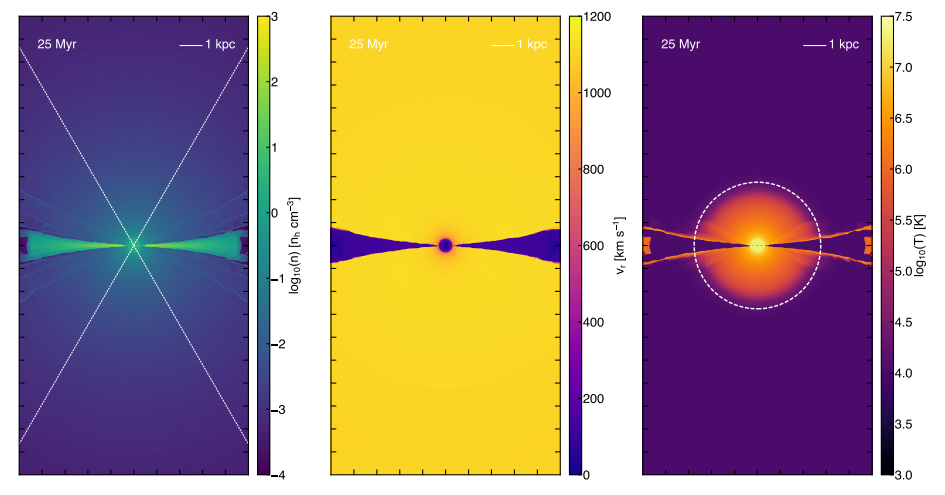
\includegraphics[width=1.0\textwidth]{plots/schneider_uniform.PNG}
    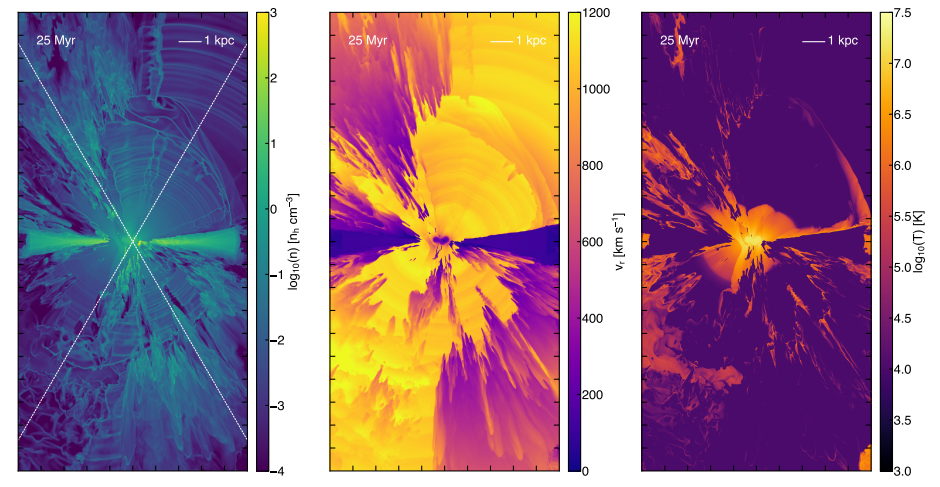
\includegraphics[width=1.0\textwidth]{plots/schneider_cluster.PNG}
    \caption{Snapshots of simulations showing an outflow that undergoes radiative cooling with two different prescriptions for feedback (i.e., energy and mass injections): uniform, central feedback (top panel), and clustered feedback (bottom panel), where energy and mass are injected randomly in small regions inside the galaxy. The galaxy is taken to be a disk, and it is noticeable in the $x - z$ plane's slices. Density, radial velocity, and temperature slices are shown on the left, central, and right panels respectively. The analytically-predicted cooling radius (eq. \ref{eq:rcool}) is plotted as a white dashed circle in the upper-right panel. Taken from Schneider et al. \citep{schneider2018production}.
    }
    \label{fig:thompson_simulation}
\end{figure}


